\documentclass[11pt]{article}

    \usepackage[breakable]{tcolorbox}
    \usepackage{parskip} % Stop auto-indenting (to mimic markdown behaviour)
    

    % Basic figure setup, for now with no caption control since it's done
    % automatically by Pandoc (which extracts ![](path) syntax from Markdown).
    \usepackage{graphicx}
    % Maintain compatibility with old templates. Remove in nbconvert 6.0
    \let\Oldincludegraphics\includegraphics
    % Ensure that by default, figures have no caption (until we provide a
    % proper Figure object with a Caption API and a way to capture that
    % in the conversion process - todo).
    \usepackage{caption}
    \DeclareCaptionFormat{nocaption}{}
    \captionsetup{format=nocaption,aboveskip=0pt,belowskip=0pt}

    \usepackage{float}
    \floatplacement{figure}{H} % forces figures to be placed at the correct location
    \usepackage{xcolor} % Allow colors to be defined
    \usepackage{enumerate} % Needed for markdown enumerations to work
    \usepackage{geometry} % Used to adjust the document margins
    \usepackage{amsmath} % Equations
    \usepackage{amssymb} % Equations
    \usepackage{textcomp} % defines textquotesingle
    % Hack from http://tex.stackexchange.com/a/47451/13684:
    \AtBeginDocument{%
        \def\PYZsq{\textquotesingle}% Upright quotes in Pygmentized code
    }
    \usepackage{upquote} % Upright quotes for verbatim code
    \usepackage{eurosym} % defines \euro

    \usepackage{iftex}
    \ifPDFTeX
        \usepackage[T1]{fontenc}
        \IfFileExists{alphabeta.sty}{
              \usepackage{alphabeta}
          }{
              \usepackage[mathletters]{ucs}
              \usepackage[utf8x]{inputenc}
          }
    \else
        \usepackage{fontspec}
        \usepackage{unicode-math}
    \fi

    \usepackage{fancyvrb} % verbatim replacement that allows latex
    \usepackage{grffile} % extends the file name processing of package graphics
                         % to support a larger range
    \makeatletter % fix for old versions of grffile with XeLaTeX
    \@ifpackagelater{grffile}{2019/11/01}
    {
      % Do nothing on new versions
    }
    {
      \def\Gread@@xetex#1{%
        \IfFileExists{"\Gin@base".bb}%
        {\Gread@eps{\Gin@base.bb}}%
        {\Gread@@xetex@aux#1}%
      }
    }
    \makeatother
    \usepackage[Export]{adjustbox} % Used to constrain images to a maximum size
    \adjustboxset{max size={0.9\linewidth}{0.9\paperheight}}

    % The hyperref package gives us a pdf with properly built
    % internal navigation ('pdf bookmarks' for the table of contents,
    % internal cross-reference links, web links for URLs, etc.)
    \usepackage{hyperref}
    % The default LaTeX title has an obnoxious amount of whitespace. By default,
    % titling removes some of it. It also provides customization options.
    \usepackage{titling}
    \usepackage{longtable} % longtable support required by pandoc >1.10
    \usepackage{booktabs}  % table support for pandoc > 1.12.2
    \usepackage{array}     % table support for pandoc >= 2.11.3
    \usepackage{calc}      % table minipage width calculation for pandoc >= 2.11.1
    \usepackage[inline]{enumitem} % IRkernel/repr support (it uses the enumerate* environment)
    \usepackage[normalem]{ulem} % ulem is needed to support strikethroughs (\sout)
                                % normalem makes italics be italics, not underlines
    \usepackage{mathrsfs}
    

    
    % Colors for the hyperref package
    \definecolor{urlcolor}{rgb}{0,.145,.698}
    \definecolor{linkcolor}{rgb}{.71,0.21,0.01}
    \definecolor{citecolor}{rgb}{.12,.54,.11}

    % ANSI colors
    \definecolor{ansi-black}{HTML}{3E424D}
    \definecolor{ansi-black-intense}{HTML}{282C36}
    \definecolor{ansi-red}{HTML}{E75C58}
    \definecolor{ansi-red-intense}{HTML}{B22B31}
    \definecolor{ansi-green}{HTML}{00A250}
    \definecolor{ansi-green-intense}{HTML}{007427}
    \definecolor{ansi-yellow}{HTML}{DDB62B}
    \definecolor{ansi-yellow-intense}{HTML}{B27D12}
    \definecolor{ansi-blue}{HTML}{208FFB}
    \definecolor{ansi-blue-intense}{HTML}{0065CA}
    \definecolor{ansi-magenta}{HTML}{D160C4}
    \definecolor{ansi-magenta-intense}{HTML}{A03196}
    \definecolor{ansi-cyan}{HTML}{60C6C8}
    \definecolor{ansi-cyan-intense}{HTML}{258F8F}
    \definecolor{ansi-white}{HTML}{C5C1B4}
    \definecolor{ansi-white-intense}{HTML}{A1A6B2}
    \definecolor{ansi-default-inverse-fg}{HTML}{FFFFFF}
    \definecolor{ansi-default-inverse-bg}{HTML}{000000}

    % common color for the border for error outputs.
    \definecolor{outerrorbackground}{HTML}{FFDFDF}

    % commands and environments needed by pandoc snippets
    % extracted from the output of `pandoc -s`
    \providecommand{\tightlist}{%
      \setlength{\itemsep}{0pt}\setlength{\parskip}{0pt}}
    \DefineVerbatimEnvironment{Highlighting}{Verbatim}{commandchars=\\\{\}}
    % Add ',fontsize=\small' for more characters per line
    \newenvironment{Shaded}{}{}
    \newcommand{\KeywordTok}[1]{\textcolor[rgb]{0.00,0.44,0.13}{\textbf{{#1}}}}
    \newcommand{\DataTypeTok}[1]{\textcolor[rgb]{0.56,0.13,0.00}{{#1}}}
    \newcommand{\DecValTok}[1]{\textcolor[rgb]{0.25,0.63,0.44}{{#1}}}
    \newcommand{\BaseNTok}[1]{\textcolor[rgb]{0.25,0.63,0.44}{{#1}}}
    \newcommand{\FloatTok}[1]{\textcolor[rgb]{0.25,0.63,0.44}{{#1}}}
    \newcommand{\CharTok}[1]{\textcolor[rgb]{0.25,0.44,0.63}{{#1}}}
    \newcommand{\StringTok}[1]{\textcolor[rgb]{0.25,0.44,0.63}{{#1}}}
    \newcommand{\CommentTok}[1]{\textcolor[rgb]{0.38,0.63,0.69}{\textit{{#1}}}}
    \newcommand{\OtherTok}[1]{\textcolor[rgb]{0.00,0.44,0.13}{{#1}}}
    \newcommand{\AlertTok}[1]{\textcolor[rgb]{1.00,0.00,0.00}{\textbf{{#1}}}}
    \newcommand{\FunctionTok}[1]{\textcolor[rgb]{0.02,0.16,0.49}{{#1}}}
    \newcommand{\RegionMarkerTok}[1]{{#1}}
    \newcommand{\ErrorTok}[1]{\textcolor[rgb]{1.00,0.00,0.00}{\textbf{{#1}}}}
    \newcommand{\NormalTok}[1]{{#1}}

    % Additional commands for more recent versions of Pandoc
    \newcommand{\ConstantTok}[1]{\textcolor[rgb]{0.53,0.00,0.00}{{#1}}}
    \newcommand{\SpecialCharTok}[1]{\textcolor[rgb]{0.25,0.44,0.63}{{#1}}}
    \newcommand{\VerbatimStringTok}[1]{\textcolor[rgb]{0.25,0.44,0.63}{{#1}}}
    \newcommand{\SpecialStringTok}[1]{\textcolor[rgb]{0.73,0.40,0.53}{{#1}}}
    \newcommand{\ImportTok}[1]{{#1}}
    \newcommand{\DocumentationTok}[1]{\textcolor[rgb]{0.73,0.13,0.13}{\textit{{#1}}}}
    \newcommand{\AnnotationTok}[1]{\textcolor[rgb]{0.38,0.63,0.69}{\textbf{\textit{{#1}}}}}
    \newcommand{\CommentVarTok}[1]{\textcolor[rgb]{0.38,0.63,0.69}{\textbf{\textit{{#1}}}}}
    \newcommand{\VariableTok}[1]{\textcolor[rgb]{0.10,0.09,0.49}{{#1}}}
    \newcommand{\ControlFlowTok}[1]{\textcolor[rgb]{0.00,0.44,0.13}{\textbf{{#1}}}}
    \newcommand{\OperatorTok}[1]{\textcolor[rgb]{0.40,0.40,0.40}{{#1}}}
    \newcommand{\BuiltInTok}[1]{{#1}}
    \newcommand{\ExtensionTok}[1]{{#1}}
    \newcommand{\PreprocessorTok}[1]{\textcolor[rgb]{0.74,0.48,0.00}{{#1}}}
    \newcommand{\AttributeTok}[1]{\textcolor[rgb]{0.49,0.56,0.16}{{#1}}}
    \newcommand{\InformationTok}[1]{\textcolor[rgb]{0.38,0.63,0.69}{\textbf{\textit{{#1}}}}}
    \newcommand{\WarningTok}[1]{\textcolor[rgb]{0.38,0.63,0.69}{\textbf{\textit{{#1}}}}}


    % Define a nice break command that doesn't care if a line doesn't already
    % exist.
    \def\br{\hspace*{\fill} \\* }
    % Math Jax compatibility definitions
    \def\gt{>}
    \def\lt{<}
    \let\Oldtex\TeX
    \let\Oldlatex\LaTeX
    \renewcommand{\TeX}{\textrm{\Oldtex}}
    \renewcommand{\LaTeX}{\textrm{\Oldlatex}}
    % Document parameters
    % Document title
    \title{raport}
    
    
    
    
    
    
    
% Pygments definitions
\makeatletter
\def\PY@reset{\let\PY@it=\relax \let\PY@bf=\relax%
    \let\PY@ul=\relax \let\PY@tc=\relax%
    \let\PY@bc=\relax \let\PY@ff=\relax}
\def\PY@tok#1{\csname PY@tok@#1\endcsname}
\def\PY@toks#1+{\ifx\relax#1\empty\else%
    \PY@tok{#1}\expandafter\PY@toks\fi}
\def\PY@do#1{\PY@bc{\PY@tc{\PY@ul{%
    \PY@it{\PY@bf{\PY@ff{#1}}}}}}}
\def\PY#1#2{\PY@reset\PY@toks#1+\relax+\PY@do{#2}}

\@namedef{PY@tok@w}{\def\PY@tc##1{\textcolor[rgb]{0.73,0.73,0.73}{##1}}}
\@namedef{PY@tok@c}{\let\PY@it=\textit\def\PY@tc##1{\textcolor[rgb]{0.24,0.48,0.48}{##1}}}
\@namedef{PY@tok@cp}{\def\PY@tc##1{\textcolor[rgb]{0.61,0.40,0.00}{##1}}}
\@namedef{PY@tok@k}{\let\PY@bf=\textbf\def\PY@tc##1{\textcolor[rgb]{0.00,0.50,0.00}{##1}}}
\@namedef{PY@tok@kp}{\def\PY@tc##1{\textcolor[rgb]{0.00,0.50,0.00}{##1}}}
\@namedef{PY@tok@kt}{\def\PY@tc##1{\textcolor[rgb]{0.69,0.00,0.25}{##1}}}
\@namedef{PY@tok@o}{\def\PY@tc##1{\textcolor[rgb]{0.40,0.40,0.40}{##1}}}
\@namedef{PY@tok@ow}{\let\PY@bf=\textbf\def\PY@tc##1{\textcolor[rgb]{0.67,0.13,1.00}{##1}}}
\@namedef{PY@tok@nb}{\def\PY@tc##1{\textcolor[rgb]{0.00,0.50,0.00}{##1}}}
\@namedef{PY@tok@nf}{\def\PY@tc##1{\textcolor[rgb]{0.00,0.00,1.00}{##1}}}
\@namedef{PY@tok@nc}{\let\PY@bf=\textbf\def\PY@tc##1{\textcolor[rgb]{0.00,0.00,1.00}{##1}}}
\@namedef{PY@tok@nn}{\let\PY@bf=\textbf\def\PY@tc##1{\textcolor[rgb]{0.00,0.00,1.00}{##1}}}
\@namedef{PY@tok@ne}{\let\PY@bf=\textbf\def\PY@tc##1{\textcolor[rgb]{0.80,0.25,0.22}{##1}}}
\@namedef{PY@tok@nv}{\def\PY@tc##1{\textcolor[rgb]{0.10,0.09,0.49}{##1}}}
\@namedef{PY@tok@no}{\def\PY@tc##1{\textcolor[rgb]{0.53,0.00,0.00}{##1}}}
\@namedef{PY@tok@nl}{\def\PY@tc##1{\textcolor[rgb]{0.46,0.46,0.00}{##1}}}
\@namedef{PY@tok@ni}{\let\PY@bf=\textbf\def\PY@tc##1{\textcolor[rgb]{0.44,0.44,0.44}{##1}}}
\@namedef{PY@tok@na}{\def\PY@tc##1{\textcolor[rgb]{0.41,0.47,0.13}{##1}}}
\@namedef{PY@tok@nt}{\let\PY@bf=\textbf\def\PY@tc##1{\textcolor[rgb]{0.00,0.50,0.00}{##1}}}
\@namedef{PY@tok@nd}{\def\PY@tc##1{\textcolor[rgb]{0.67,0.13,1.00}{##1}}}
\@namedef{PY@tok@s}{\def\PY@tc##1{\textcolor[rgb]{0.73,0.13,0.13}{##1}}}
\@namedef{PY@tok@sd}{\let\PY@it=\textit\def\PY@tc##1{\textcolor[rgb]{0.73,0.13,0.13}{##1}}}
\@namedef{PY@tok@si}{\let\PY@bf=\textbf\def\PY@tc##1{\textcolor[rgb]{0.64,0.35,0.47}{##1}}}
\@namedef{PY@tok@se}{\let\PY@bf=\textbf\def\PY@tc##1{\textcolor[rgb]{0.67,0.36,0.12}{##1}}}
\@namedef{PY@tok@sr}{\def\PY@tc##1{\textcolor[rgb]{0.64,0.35,0.47}{##1}}}
\@namedef{PY@tok@ss}{\def\PY@tc##1{\textcolor[rgb]{0.10,0.09,0.49}{##1}}}
\@namedef{PY@tok@sx}{\def\PY@tc##1{\textcolor[rgb]{0.00,0.50,0.00}{##1}}}
\@namedef{PY@tok@m}{\def\PY@tc##1{\textcolor[rgb]{0.40,0.40,0.40}{##1}}}
\@namedef{PY@tok@gh}{\let\PY@bf=\textbf\def\PY@tc##1{\textcolor[rgb]{0.00,0.00,0.50}{##1}}}
\@namedef{PY@tok@gu}{\let\PY@bf=\textbf\def\PY@tc##1{\textcolor[rgb]{0.50,0.00,0.50}{##1}}}
\@namedef{PY@tok@gd}{\def\PY@tc##1{\textcolor[rgb]{0.63,0.00,0.00}{##1}}}
\@namedef{PY@tok@gi}{\def\PY@tc##1{\textcolor[rgb]{0.00,0.52,0.00}{##1}}}
\@namedef{PY@tok@gr}{\def\PY@tc##1{\textcolor[rgb]{0.89,0.00,0.00}{##1}}}
\@namedef{PY@tok@ge}{\let\PY@it=\textit}
\@namedef{PY@tok@gs}{\let\PY@bf=\textbf}
\@namedef{PY@tok@gp}{\let\PY@bf=\textbf\def\PY@tc##1{\textcolor[rgb]{0.00,0.00,0.50}{##1}}}
\@namedef{PY@tok@go}{\def\PY@tc##1{\textcolor[rgb]{0.44,0.44,0.44}{##1}}}
\@namedef{PY@tok@gt}{\def\PY@tc##1{\textcolor[rgb]{0.00,0.27,0.87}{##1}}}
\@namedef{PY@tok@err}{\def\PY@bc##1{{\setlength{\fboxsep}{\string -\fboxrule}\fcolorbox[rgb]{1.00,0.00,0.00}{1,1,1}{\strut ##1}}}}
\@namedef{PY@tok@kc}{\let\PY@bf=\textbf\def\PY@tc##1{\textcolor[rgb]{0.00,0.50,0.00}{##1}}}
\@namedef{PY@tok@kd}{\let\PY@bf=\textbf\def\PY@tc##1{\textcolor[rgb]{0.00,0.50,0.00}{##1}}}
\@namedef{PY@tok@kn}{\let\PY@bf=\textbf\def\PY@tc##1{\textcolor[rgb]{0.00,0.50,0.00}{##1}}}
\@namedef{PY@tok@kr}{\let\PY@bf=\textbf\def\PY@tc##1{\textcolor[rgb]{0.00,0.50,0.00}{##1}}}
\@namedef{PY@tok@bp}{\def\PY@tc##1{\textcolor[rgb]{0.00,0.50,0.00}{##1}}}
\@namedef{PY@tok@fm}{\def\PY@tc##1{\textcolor[rgb]{0.00,0.00,1.00}{##1}}}
\@namedef{PY@tok@vc}{\def\PY@tc##1{\textcolor[rgb]{0.10,0.09,0.49}{##1}}}
\@namedef{PY@tok@vg}{\def\PY@tc##1{\textcolor[rgb]{0.10,0.09,0.49}{##1}}}
\@namedef{PY@tok@vi}{\def\PY@tc##1{\textcolor[rgb]{0.10,0.09,0.49}{##1}}}
\@namedef{PY@tok@vm}{\def\PY@tc##1{\textcolor[rgb]{0.10,0.09,0.49}{##1}}}
\@namedef{PY@tok@sa}{\def\PY@tc##1{\textcolor[rgb]{0.73,0.13,0.13}{##1}}}
\@namedef{PY@tok@sb}{\def\PY@tc##1{\textcolor[rgb]{0.73,0.13,0.13}{##1}}}
\@namedef{PY@tok@sc}{\def\PY@tc##1{\textcolor[rgb]{0.73,0.13,0.13}{##1}}}
\@namedef{PY@tok@dl}{\def\PY@tc##1{\textcolor[rgb]{0.73,0.13,0.13}{##1}}}
\@namedef{PY@tok@s2}{\def\PY@tc##1{\textcolor[rgb]{0.73,0.13,0.13}{##1}}}
\@namedef{PY@tok@sh}{\def\PY@tc##1{\textcolor[rgb]{0.73,0.13,0.13}{##1}}}
\@namedef{PY@tok@s1}{\def\PY@tc##1{\textcolor[rgb]{0.73,0.13,0.13}{##1}}}
\@namedef{PY@tok@mb}{\def\PY@tc##1{\textcolor[rgb]{0.40,0.40,0.40}{##1}}}
\@namedef{PY@tok@mf}{\def\PY@tc##1{\textcolor[rgb]{0.40,0.40,0.40}{##1}}}
\@namedef{PY@tok@mh}{\def\PY@tc##1{\textcolor[rgb]{0.40,0.40,0.40}{##1}}}
\@namedef{PY@tok@mi}{\def\PY@tc##1{\textcolor[rgb]{0.40,0.40,0.40}{##1}}}
\@namedef{PY@tok@il}{\def\PY@tc##1{\textcolor[rgb]{0.40,0.40,0.40}{##1}}}
\@namedef{PY@tok@mo}{\def\PY@tc##1{\textcolor[rgb]{0.40,0.40,0.40}{##1}}}
\@namedef{PY@tok@ch}{\let\PY@it=\textit\def\PY@tc##1{\textcolor[rgb]{0.24,0.48,0.48}{##1}}}
\@namedef{PY@tok@cm}{\let\PY@it=\textit\def\PY@tc##1{\textcolor[rgb]{0.24,0.48,0.48}{##1}}}
\@namedef{PY@tok@cpf}{\let\PY@it=\textit\def\PY@tc##1{\textcolor[rgb]{0.24,0.48,0.48}{##1}}}
\@namedef{PY@tok@c1}{\let\PY@it=\textit\def\PY@tc##1{\textcolor[rgb]{0.24,0.48,0.48}{##1}}}
\@namedef{PY@tok@cs}{\let\PY@it=\textit\def\PY@tc##1{\textcolor[rgb]{0.24,0.48,0.48}{##1}}}

\def\PYZbs{\char`\\}
\def\PYZus{\char`\_}
\def\PYZob{\char`\{}
\def\PYZcb{\char`\}}
\def\PYZca{\char`\^}
\def\PYZam{\char`\&}
\def\PYZlt{\char`\<}
\def\PYZgt{\char`\>}
\def\PYZsh{\char`\#}
\def\PYZpc{\char`\%}
\def\PYZdl{\char`\$}
\def\PYZhy{\char`\-}
\def\PYZsq{\char`\'}
\def\PYZdq{\char`\"}
\def\PYZti{\char`\~}
% for compatibility with earlier versions
\def\PYZat{@}
\def\PYZlb{[}
\def\PYZrb{]}
\makeatother


    % For linebreaks inside Verbatim environment from package fancyvrb.
    \makeatletter
        \newbox\Wrappedcontinuationbox
        \newbox\Wrappedvisiblespacebox
        \newcommand*\Wrappedvisiblespace {\textcolor{red}{\textvisiblespace}}
        \newcommand*\Wrappedcontinuationsymbol {\textcolor{red}{\llap{\tiny$\m@th\hookrightarrow$}}}
        \newcommand*\Wrappedcontinuationindent {3ex }
        \newcommand*\Wrappedafterbreak {\kern\Wrappedcontinuationindent\copy\Wrappedcontinuationbox}
        % Take advantage of the already applied Pygments mark-up to insert
        % potential linebreaks for TeX processing.
        %        {, <, #, %, $, ' and ": go to next line.
        %        _, }, ^, &, >, - and ~: stay at end of broken line.
        % Use of \textquotesingle for straight quote.
        \newcommand*\Wrappedbreaksatspecials {%
            \def\PYGZus{\discretionary{\char`\_}{\Wrappedafterbreak}{\char`\_}}%
            \def\PYGZob{\discretionary{}{\Wrappedafterbreak\char`\{}{\char`\{}}%
            \def\PYGZcb{\discretionary{\char`\}}{\Wrappedafterbreak}{\char`\}}}%
            \def\PYGZca{\discretionary{\char`\^}{\Wrappedafterbreak}{\char`\^}}%
            \def\PYGZam{\discretionary{\char`\&}{\Wrappedafterbreak}{\char`\&}}%
            \def\PYGZlt{\discretionary{}{\Wrappedafterbreak\char`\<}{\char`\<}}%
            \def\PYGZgt{\discretionary{\char`\>}{\Wrappedafterbreak}{\char`\>}}%
            \def\PYGZsh{\discretionary{}{\Wrappedafterbreak\char`\#}{\char`\#}}%
            \def\PYGZpc{\discretionary{}{\Wrappedafterbreak\char`\%}{\char`\%}}%
            \def\PYGZdl{\discretionary{}{\Wrappedafterbreak\char`\$}{\char`\$}}%
            \def\PYGZhy{\discretionary{\char`\-}{\Wrappedafterbreak}{\char`\-}}%
            \def\PYGZsq{\discretionary{}{\Wrappedafterbreak\textquotesingle}{\textquotesingle}}%
            \def\PYGZdq{\discretionary{}{\Wrappedafterbreak\char`\"}{\char`\"}}%
            \def\PYGZti{\discretionary{\char`\~}{\Wrappedafterbreak}{\char`\~}}%
        }
        % Some characters . , ; ? ! / are not pygmentized.
        % This macro makes them "active" and they will insert potential linebreaks
        \newcommand*\Wrappedbreaksatpunct {%
            \lccode`\~`\.\lowercase{\def~}{\discretionary{\hbox{\char`\.}}{\Wrappedafterbreak}{\hbox{\char`\.}}}%
            \lccode`\~`\,\lowercase{\def~}{\discretionary{\hbox{\char`\,}}{\Wrappedafterbreak}{\hbox{\char`\,}}}%
            \lccode`\~`\;\lowercase{\def~}{\discretionary{\hbox{\char`\;}}{\Wrappedafterbreak}{\hbox{\char`\;}}}%
            \lccode`\~`\:\lowercase{\def~}{\discretionary{\hbox{\char`\:}}{\Wrappedafterbreak}{\hbox{\char`\:}}}%
            \lccode`\~`\?\lowercase{\def~}{\discretionary{\hbox{\char`\?}}{\Wrappedafterbreak}{\hbox{\char`\?}}}%
            \lccode`\~`\!\lowercase{\def~}{\discretionary{\hbox{\char`\!}}{\Wrappedafterbreak}{\hbox{\char`\!}}}%
            \lccode`\~`\/\lowercase{\def~}{\discretionary{\hbox{\char`\/}}{\Wrappedafterbreak}{\hbox{\char`\/}}}%
            \catcode`\.\active
            \catcode`\,\active
            \catcode`\;\active
            \catcode`\:\active
            \catcode`\?\active
            \catcode`\!\active
            \catcode`\/\active
            \lccode`\~`\~
        }
    \makeatother

    \let\OriginalVerbatim=\Verbatim
    \makeatletter
    \renewcommand{\Verbatim}[1][1]{%
        %\parskip\z@skip
        \sbox\Wrappedcontinuationbox {\Wrappedcontinuationsymbol}%
        \sbox\Wrappedvisiblespacebox {\FV@SetupFont\Wrappedvisiblespace}%
        \def\FancyVerbFormatLine ##1{\hsize\linewidth
            \vtop{\raggedright\hyphenpenalty\z@\exhyphenpenalty\z@
                \doublehyphendemerits\z@\finalhyphendemerits\z@
                \strut ##1\strut}%
        }%
        % If the linebreak is at a space, the latter will be displayed as visible
        % space at end of first line, and a continuation symbol starts next line.
        % Stretch/shrink are however usually zero for typewriter font.
        \def\FV@Space {%
            \nobreak\hskip\z@ plus\fontdimen3\font minus\fontdimen4\font
            \discretionary{\copy\Wrappedvisiblespacebox}{\Wrappedafterbreak}
            {\kern\fontdimen2\font}%
        }%

        % Allow breaks at special characters using \PYG... macros.
        \Wrappedbreaksatspecials
        % Breaks at punctuation characters . , ; ? ! and / need catcode=\active
        \OriginalVerbatim[#1,codes*=\Wrappedbreaksatpunct]%
    }
    \makeatother

    % Exact colors from NB
    \definecolor{incolor}{HTML}{303F9F}
    \definecolor{outcolor}{HTML}{D84315}
    \definecolor{cellborder}{HTML}{CFCFCF}
    \definecolor{cellbackground}{HTML}{F7F7F7}

    % prompt
    \makeatletter
    \newcommand{\boxspacing}{\kern\kvtcb@left@rule\kern\kvtcb@boxsep}
    \makeatother
    \newcommand{\prompt}[4]{
        {\ttfamily\llap{{\color{#2}[#3]:\hspace{3pt}#4}}\vspace{-\baselineskip}}
    }
    

    
    % Prevent overflowing lines due to hard-to-break entities
    \sloppy
    % Setup hyperref package
    \hypersetup{
      breaklinks=true,  % so long urls are correctly broken across lines
      colorlinks=true,
      urlcolor=urlcolor,
      linkcolor=linkcolor,
      citecolor=citecolor,
      }
    % Slightly bigger margins than the latex defaults
    
    \geometry{verbose,tmargin=1in,bmargin=1in,lmargin=1in,rmargin=1in}
    
    

\begin{document}
    
    \maketitle
    
    

    
    \hypertarget{dont-get-kicked---machine-learning-classification-problem}{%
\section{\texorpdfstring{\emph{Don't get kicked} - Machine Learning
Classification
Problem}{Don't get kicked - Machine Learning Classification Problem}}\label{dont-get-kicked---machine-learning-classification-problem}}

Projekt realizowany w ramach przedmiotu \emph{Warsztaty Badawcze},
kierunku Inżynieria i Analiza Danych na wydziale Matematyki i Nauk
Informacyjnych Politechniki Warszawskiej, pod opieką merytoryczną mgr
inż. \textbf{Mateusza Chilińskiego}.

Autorzy: \textbf{Maciej Borkowski, Mateusz Kubita, Tymoteusz Kwieciński}

    \hypertarget{cel-zadania-i-problem-biznesowy}{%
\section{Cel zadania i problem
biznesowy}\label{cel-zadania-i-problem-biznesowy}}

Naszym zadaniem biznesowym zostało przygotowanie modelu uczenia
maszynowego, który pozwoliłby kategoryzować używane samochody
sprzedawane na giełdzie aut. Samochody miały zostać przyporządkowane do
jednej z dwóch kategorii - \emph{bezpieczny zakup} oraz
\emph{nieopłacalny zakup} - w środowisku handlarzy aut na takie
samochody mówi się \emph{cytryny} (z ang. \emph{lemon}).

Zadanie zostało zaproponowane w formie zawodów w serwisie \emph{kaggle}.
Niestety, w momencie kiedy dołączyliśmy do zawodów, nie można było
składać nowych rankingowych zgłoszeń, a jedynie porównywać swoje wyniki
do zbioru testowego za pomocą algorytmu serwisu. Link do zawodów:
\url{https://www.kaggle.com/competitions/DontGetKicked}.

Nasza ocena, czy sprzedawany samochód jest zakupem nieopłacalnym, miała
być dokonywana na podstawie różnych jego cech uporządkowanych w formie
tabelarycznej. Algorytm wyuczony na przygotowanych danych treningowych
miałby później służyć do wykrywania ryzykownych zakupów w trakcie
prowadzenia aukcji. Wobec tego przyjeliśmy dwa główne założenia, które
powinien spełniać tak wytrenowany przez nas model: 1. model powinien być
w miarę możliwości \textbf{wyjaśnialny} - uznaliśmy, że nie byłoby
wskazane, aby model używany przez sprzedawców był tak zwaną \emph{czarną
skrzynką}, po prostu wypluwającą oceny na podstawie nieznanych
przesłanek. W wielu przypadkach sprzedaż samochodów opiera się na
intuicji oraz wieloletnim doświadczeniu w zawodzie sprzedawcy. 2.
ważniejsze dla nas jest \textbf{wykrycie nieopłacalnych zakupów} -
nadmierne przyporządkowanie do kategorii fałszywie pozytywnych nie
byłoby aż tak bardzo kosztowne dla naszych klientów. Jest to w miare
logiczna obserwacja, bo w takich przypadkach lepiej dmuchać na zimne i
zakwalifikować więcej ryzykownych samochodów, które potencjalnie nasz
klient może kupić, do kategorii \emph{nieopłacalny zakup}. W przypadku
zakupu samochodu bardzo ryzykownego, handlarz auto może nie tylko nie
zarobić, ale również stracić duże pieniądze.

Naszym celem wobec tego nie było jedynie uzyskanie jak najlepszych
rezultatów w zawodach, ale również przygotowanie modelu, który miałby
zastosowanie w rzeczywistości.

Z tak zdefiniowanymi celami przeszliśmy do wstępnej, eksploracyjnej
analizy dostarczonych nam danych zawierających informacje o zakupionych
samochodach w przeszłości, a także do ich preprocessingu.

    \hypertarget{eksploracyjna-analiza-danych-oraz-preprocessing}{%
\section{Eksploracyjna analiza danych oraz
preprocessing}\label{eksploracyjna-analiza-danych-oraz-preprocessing}}

Nasz zbiór danych zawiera 33 kolumny, co wiązało się z dość obszernym
preprocessingiem. Do każdej kolumny podeszliśmy indywidualnie, zarówno
podczas analizy danych i preprocessingu - odpowiednio transformując jej
wartości, dostosowując do algorytmów uczenia maszynowego.

Na podstawie eksploracji danych (m.in. wizualizacji rozkładów, analizy
korelacji i przeglądu kategorii) wybraliśmy podzbiór kolumn zawierający
jak najwięcej kluczowych informacji i jednocześnie prostych do
zakodowania, utworzyliśmy ponadto nowe kolumny wyciągając istotne
informacje z pozostałych, takie jak pora roku, w której samochód został
zakupiony, liczba drzwi czy rodzaj nadwozia.

Dokonaliśmy imputacji braków danych różnymi metodami - średnią, medianą,
tworząc oddzielną kategorię czy zaznaczając tę informacje w nowej
kolumnie.

W przypadku kolumn kategorycznych zazwyczaj decydowaliśmy się na użycie
algorytmu \texttt{OneHotEncoding} z pakietu \texttt{scikit-learn}. Jest
to dość intuicyjna metoda, dzięki której nie tracimy żadnych informacji.
Dodaje on do zbioru danych dodatkowe kolumny (ich liczność jest
odpowiednia liczbą kategorii), a następnie daje wartość 1 tam, gdzie
jest odpowiednia kategoria. Sprawia to, że informacje te są zakodowane w
postaci liczbowej. Niestety sprawia to również, że dodajemy wiele
dodatkowych kolumn, co negatywnie wpływa na interpretowalność modelu i
pogarszamy wydajność. Przykładowymi kolumnami kategorycznymi, na których
zastosowaliśmy ten algorytm są \texttt{TopThreeAmericanName},
\texttt{WheelTypeID},\texttt{Nationality}, itd\ldots{}

Kolejnym ważnym etapem preprocessingu była standaryzacja danych.
Zważając na fakt, że budowaliśmy modele które są czułe na skale
zmiennych (np. SVM czy regresja logistyczna) musieliśmy wszystkie
wartości liczbowe w jakiś sposób przeskalować, aby były między sobą
`porównywalne'. Zastosowaliśmy klasę \texttt{StandardScaler}, która
odejmuje od każdej wartości średnią arytmetyczną, a następnie dzieli
przez wariancję. Przykładowymi kolumnami objętymi tym algorytmem są:
\texttt{VehOdo},\texttt{VehBCost}, \texttt{WarrantyCost}, itd \ldots{}

Zbiór danych do budowy dostępnych w witrynie \emph{kaggle} podzieliliśmy
przed rozpoczęciem analizy na zbiór treningowy oraz walidacyjny,
korzystając ze stratyfikacji targetu - z uwagi na to, że klasa o
wartości 1 była niedoreprezentowana, musieliśmy zrobić wszystko, aby
podział zbioru był jak najlepszy.

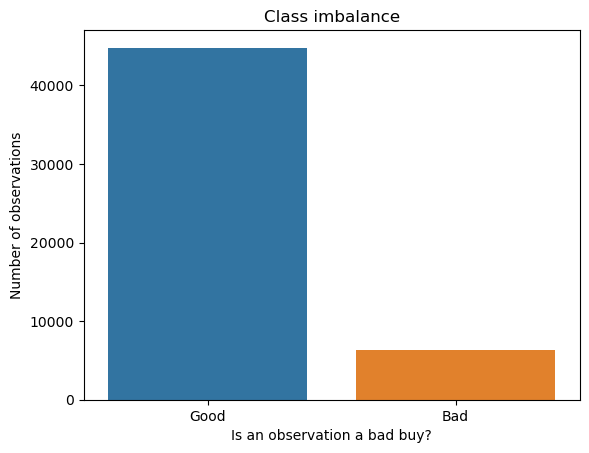
\includegraphics{plots/class imbalance.png}

W trakcie dalszej pracy nad projektem, np. już w trakcie budowania
modelów wielokrotnie wracaliśmy do etapu preprocesingu, gdyż okazało
się, że mamy nowe pomysły na przygotowanie danych lub odkryliśmy nowe,
ciekawe zależności w danych. Jedną z najbardziej widowiskowych zmian
udało się odnaleźć na etapie
\hyperref[ocena-predykcyjności-cech]{weryfikacji istotności cech} w
modelu lasów losowych. Okazało się, że bardzo istotnym elementem
preprocessingu jest odizolowanie braków danych w zmiennej
\texttt{WheelTypeID} do nowej zmiennej w ramach metody
\texttt{OneHotEncoding}, gdyż znaczna część obserwacji posiadających
brak danych w tej kolumnie była złym zakupem.

    \hypertarget{modele}{%
\section{Modele}\label{modele}}

    \hypertarget{logistic-regression}{%
\section{Logistic regression}\label{logistic-regression}}

\hypertarget{opis-dziaux142ania}{%
\subsubsection{Opis działania}\label{opis-dziaux142ania}}

Regresja logistyczna służy najczęściej do szacowania prawdopodobieństwa
przynależności przykładu do określonej klasy. Jeśli oszacowane
prawdopodobieństwo przekracza 50\%, to model prognozuje, że próbka ta
należy do np. klasy pozytywnej, zaś w przeciwnym przypadku do klasy
negatywnej. Podobnie jak w przypadku regresji liniowej w modelu regresji
logistycznej wyliczana jest ważona suma cech wejściowych. Nie są jednak
wyświetlane bezpośrednie wyniki, lecz rezultat tzw. funkcji
logistycznej.

\hypertarget{przygotowanie-modelu}{%
\subsubsection{Przygotowanie modelu}\label{przygotowanie-modelu}}

Pierwszy wytrenowany model uzyskał wynik 89.5\% dokładności oraz 70.95\%
precyzji na zbiorze walidacyjnym. Bardzo podobne rezultaty otrzymaliśmy
na zbiorze treningowym, więc model nie przejawia oznak przetrenowania.
Nie są to jednak bardzo zadowalające wyniki.

Przetestowaliśmy również parametr class\_weight z wartością `balanced'
ze względu na niezbalansowany charakter zmiennej objaśnianej, jednak
pogorszyło to rezultaty modelu.

Następnie zajęliśmy się regularyzacją modelu regresji logistycznej -
wyboru regresji grzbietowej lub regresji metodą LASSO oraz najlepszego
współczynnika regularyzacji C za pomocą przeszukiwania siatki
hiperparametrów na podstawie dokładności. Regularyzacja nieznacznie
poprawiła rezultaty modelu.

Znaczną poprawę prezycji do 75.56\% otrzymaliśmy stosując wielomianową
regresję drugiego rzędu, ponadto model ten osiągnął najlepszy rezultat
gini.

\begin{figure}
\centering
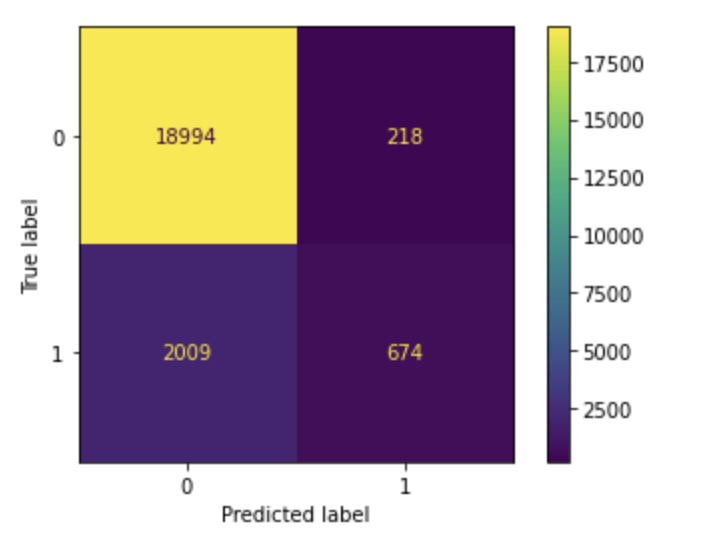
\includegraphics{plots/reg_confusion.png}
\caption{reg\_coef}
\end{figure}

\hypertarget{wizualizacje}{%
\subsubsection{Wizualizacje}\label{wizualizacje}}

Współczynnik istotności cech funkcji decyzyjnej pozwala nam
zaobserwować, które kolumny miały największe znaczenie przy podejmowanej
przez model dezycji:

\begin{figure}
\centering
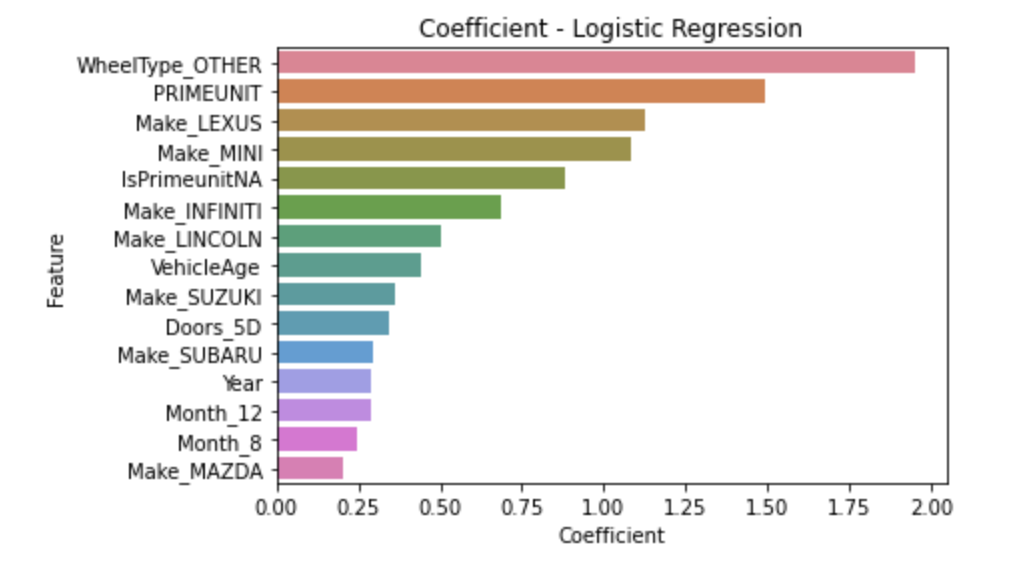
\includegraphics{plots/reg_coef.png}
\caption{reg\_coef}
\end{figure}

Dane pochodzą z modelu reularyzowanego za pomocą grid search.
Obserwujemy, że największe znaczenie w modelu miał brak informacji o
typie opon samochodu, a następnie informacja, czy na samodchód będzie
większy popyt. Widać, że model wyraźnie `skupiał się' również na
niektórych markach samochodów.

Najlepsze rezultaty gini oraz krzywe roc osiągnął model wielomianowej
regresji:

Dla danych treningowych: gini = 0.6167

\begin{figure}
\centering
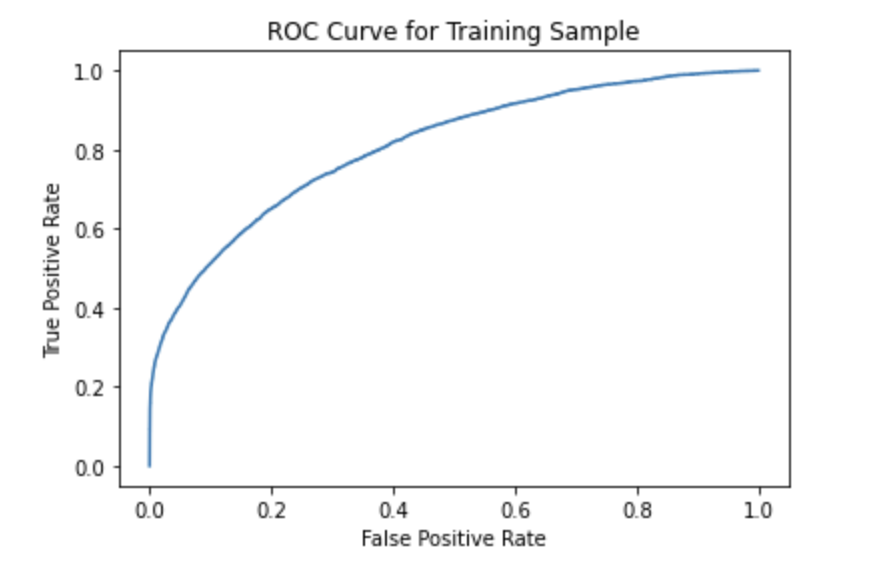
\includegraphics{plots/reg_roc_train.png}
\caption{reg\_coef}
\end{figure}

Dla danych walidacyjnych: gini = 0.5217

\begin{figure}
\centering
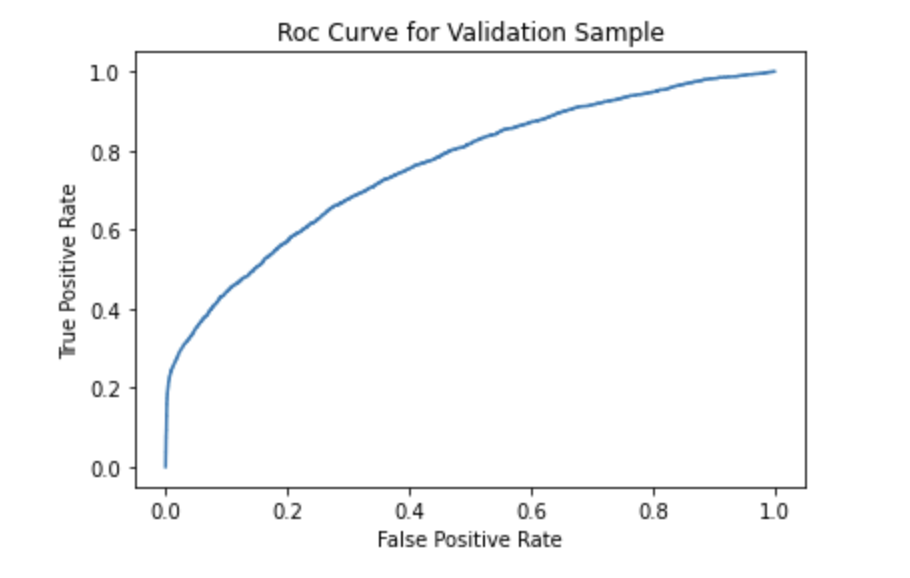
\includegraphics{plots/reg_roc_val.png}
\caption{reg\_coef}
\end{figure}

\hypertarget{podsumowanie}{%
\subsubsection{Podsumowanie}\label{podsumowanie}}

Ostatecznie musimy przyznać, że rezultaty osiągane przez regresję
logistyczną nie są bardzo zadowalające. Stanowią natomiast dobrą
podstawę do wykorzystania w klasyfikatorze głosującym.

    \hypertarget{decision-tree}{%
\section{Decision tree}\label{decision-tree}}

\hypertarget{opis-dziaux142ania}{%
\subsubsection{Opis działania}\label{opis-dziaux142ania}}

Algorytm drzewa decyzyjnego polega na tworzeniu modelu predykcyjnego w
formie struktury drzewa. Na początku, na podstawie dostępnych danych
treningowych, algorytm szuka najlepszego podziału zbioru danych na
podstawie wybranych cech. Następnie, na podstawie kryteriów decyzyjnych,
takich jak entropia czy wskaźnik Giniego, tworzona jest struktura
drzewa, gdzie wierzchołki reprezentują decyzje, a krawędzie oznaczają
możliwe wartości cech. Ostatecznie, drzewo decyzyjne może być
wykorzystane do klasyfikacji nowych, nieznanych danych poprzez
przechodzenie przez strukturę drzewa na podstawie wartości cech tych
danych.

\hypertarget{przygotowanie-modelu}{%
\subsubsection{Przygotowanie modelu}\label{przygotowanie-modelu}}

Pierwszy przygotowany model drzewa decyzyjnego bez regularyzacji
hiperparametrów został przetrenowany - model dopasował się idelanie do
danych treningowych.

Dokonaliśmy przeszukiwania siatki hiperparametrów: maksymalnej
głębokości, maksymalnej liczbie cech uwzględnianej przy popdziale,
minimalnej liczbie próbek znajdującej się w liściu oraz minimalnej
liczbie próbek, jakie muszą znajdować się w węźle przed podziałem. Do
przeszukiwania siatki wykorzystaliśmy klasę \texttt{RandomizedSearchCV}
ze skupieniem się ponownie na znajdowaniu najlepszej dokładności.

Rezultaty regularyzacji okazały się satysfakcjonujące, uzyskaliśmy
89.95\% dokładności oraz 81.46\% precyzji na zbiorze walidacyjnym,
natomiast w tym przypadku model się nie przetrenowuje.

\begin{figure}
\centering
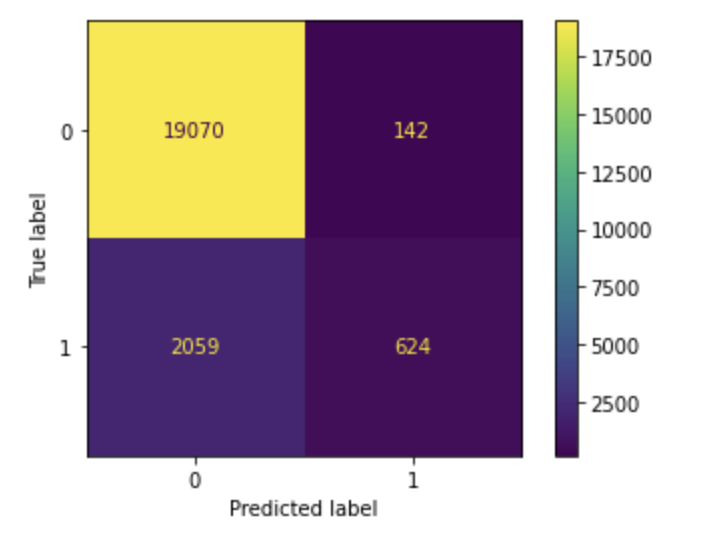
\includegraphics{plots/dct_confusion.png}
\caption{reg\_coef}
\end{figure}

\hypertarget{wizualizacje}{%
\subsubsection{Wizualizacje}\label{wizualizacje}}

Atrybut feature\_importance drzewa decyzyjnego pozwala nam określić, jak
bardzo poszczególne cechy przyczyniają się do podejmowania decyzji w
modelu. W regularyzowanym modelu drzewa decyzyjnego wyraźnie kluczową
cechą okazał się brak danych dla typu koła:

\begin{figure}
\centering
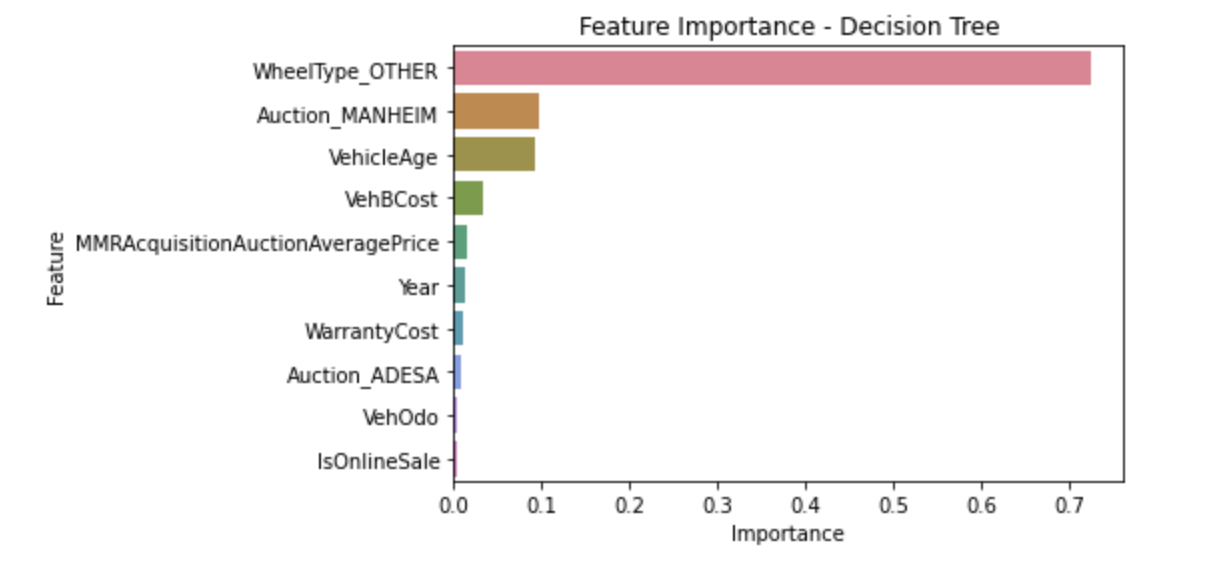
\includegraphics{plots/dct_feature_importance.png}
\caption{reg\_coef}
\end{figure}

Niestety dla drzewa decyzyjnego nie otrzymujemy zatysfakcjonującego
wyniku gini i krzywych roc:

Dla danych treningowych: gini = 0.4644

\begin{figure}
\centering
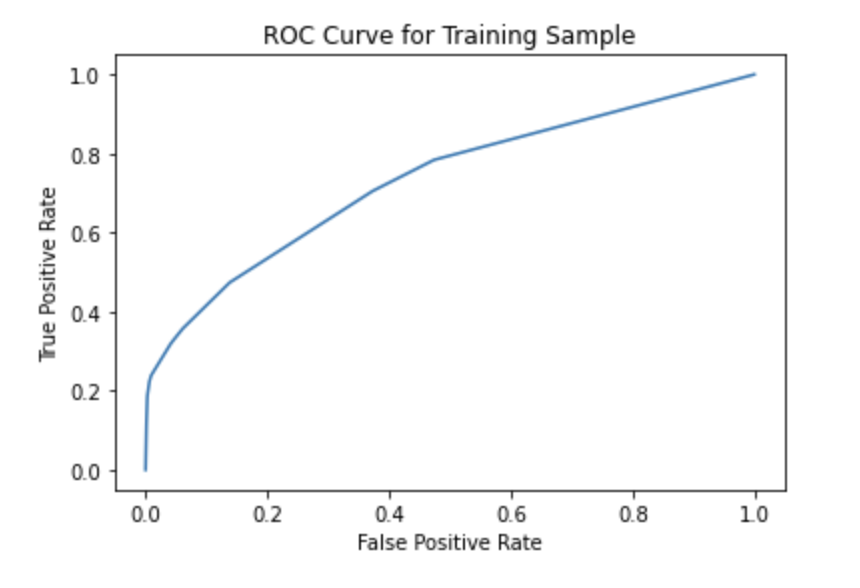
\includegraphics{plots/dct_roc_train.png}
\caption{reg\_coef}
\end{figure}

Dla danych walidacyjnych: gini = 0.4343

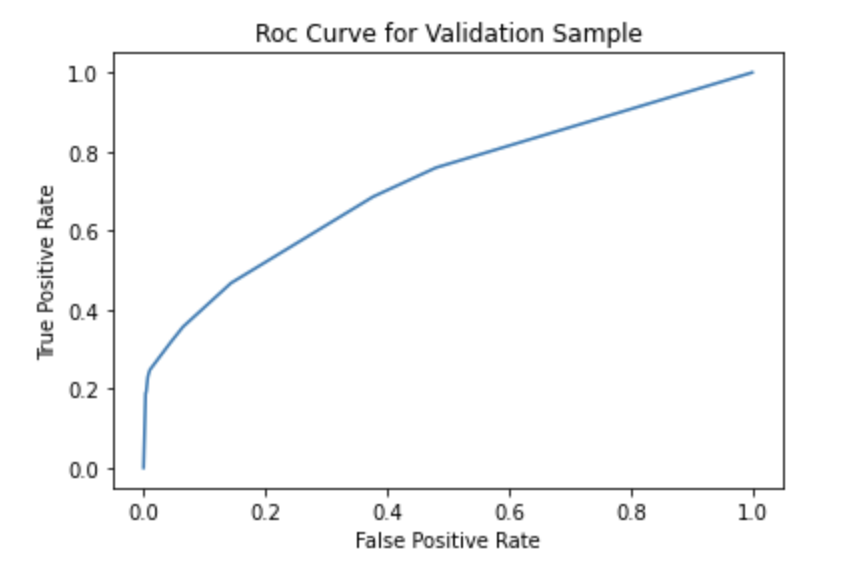
\includegraphics{plots/dct_roc_val.png}

\hypertarget{podsumowanie}{%
\subsubsection{Podsumowanie}\label{podsumowanie}}

W porównaniu do modelu regresji logistycznej otrzymaliśmy podobną
dokładność i dużo lepszą precyzję stosujac drzewo decyzyjne. Dużo gorzej
jednak wypadł wynik gini. Ponownie będziemy mogli wykorzystać rezultaty
z drzewa decyzyjnego przy klasyfikatorze głosującym.

    \hypertarget{knn-classifier}{%
\section{KNN classifier}\label{knn-classifier}}

\hypertarget{opis-dziaux142ania}{%
\subsubsection{Opis działania}\label{opis-dziaux142ania}}

Algorytm KNN Classifier polega na klasyfikowaniu nowej próbki poprzez
porównanie jej z \texttt{k} najbliższymi sąsiadami ze zbioru
treningowego na podstawie obliczonych odległości (np. euklidesowej)
między nimi. Decyzję o przyporządkowaniu nowej obserwacji do klasy
najczęściej podejmuje się na podstawie głosowania większościowego lub
najkrótszych odległości między centroidami.

\hypertarget{przygotowanie-modelu}{%
\subsubsection{Przygotowanie modelu}\label{przygotowanie-modelu}}

Po wykonaniu hiperparametryzacji za pomocą metody grid search
sprawdziliśmy jak sprawuje się model na wydzielonym zbiorze
walidacyjnym.

\begin{figure}
\centering
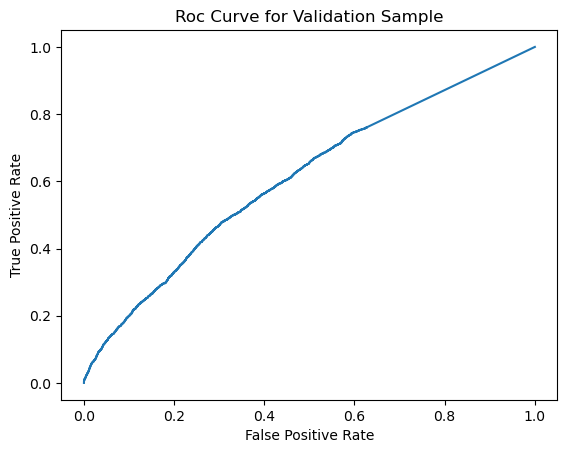
\includegraphics{plots/KNN_roc.png}
\caption{roc curve}
\end{figure}

Krzywa ROC dla modelu KNN, na zbiorze walidacyjnym.

Niestety jak się okazało, model nie sprawuje się zbyt dobrze. Otrzymana
wartość indeksu gini dla zbioru walidacyjnego to zaledwie
\texttt{0.3332}.

\hypertarget{redukcja-wielowymiarowoux15bci}{%
\subsubsection{Redukcja
wielowymiarowości}\label{redukcja-wielowymiarowoux15bci}}

Model KNN sprawuje się dużo gorzej przy wielu wymiarach. W związku z tym
postanowiliśmy zredukować liczbę wymiarów naszego zbioru danych. Z
pomocą przyszedł nam algorytm PCA, który zastosowaliśmy do tego zadania.

Po odpowiednim przygotowaniu danych postanowiliśmy wybrać liczbę
wymiarów do której ten algorytm będzie skalować nasze danę, aby zachować
dostatecznie dużo informacji, przy jednoczesnej redukcji wymiarów. W
związku z tym ustaliliśmy, że należy ograniczyć liczbę wymiarów tak aby
łączna wariancja miała wartość co najmniej 95\%.

\begin{figure}
\centering
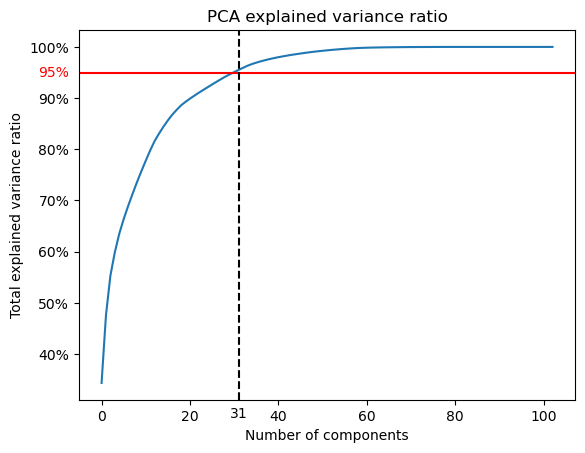
\includegraphics{plots/PCA_variance.png}
\caption{pca}
\end{figure}

Ustatliliśmy docelową liczbę wymiarów jako 31 - co wydawało się
rozsądnym balansem pomiędzy utratą informacji, a redukcją wymiarów.
Zbiór danych w wyniku preprocessingu uwzględniającego m.in. One-Hot
encoding, a także innych operacji zwiększające liczbę wymiarów danych
spowodowały, że ramka zawierała 103 wymiary.

Okazało się jednak, że zastosowana redukcja wymiarów nie przyniosła
satysfakcjonujących rezultatów, w kwestii wydajności modelu gdyż model
po redukcji wymiarów sprawował się gorzej niż przed, co widać na
załączonym wykresie krzywej ROC.

\begin{figure}
\centering
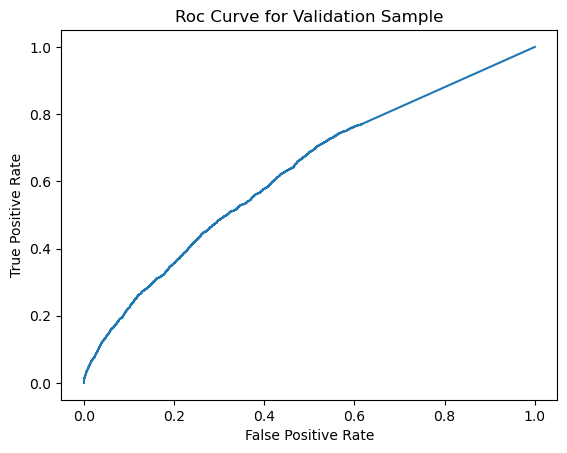
\includegraphics{plots/KNN_pca_roc.png}
\caption{roc curve}
\end{figure}

Wskaźnik gini spadł do około \texttt{0.25}, co wydawało nam się całkiem
sporą różnicą. Zdecydowaliśmy, że model nie sprawował się lepiej od tego
przed zastosowaniem PCA, chyba że wziąć pod uwagę czas jego działania.
Algorytm KNN operujący na zmodyfikowanym zbiorze danych działał
szybciej, ale przyspieszenie algorytmu nie było naszym celem.

Macierz pomyłek dla modelu przed redukcją wymiarów:

\begin{figure}
\centering
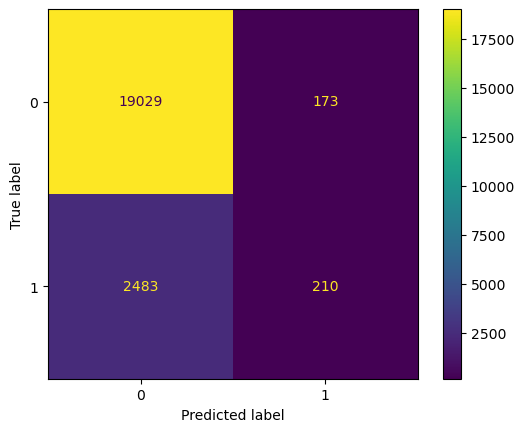
\includegraphics{plots/KNN_confusion.png}
\caption{conf\_knn}
\end{figure}

Wynik algorytmu na danych testowych z kaggla:

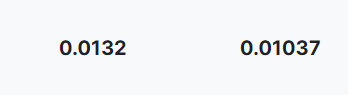
\includegraphics{plots/KNN_res.png}

\hypertarget{podsumowanie}{%
\subsubsection{Podsumowanie}\label{podsumowanie}}

\textbf{Ogólnie model ten poradził sobie raczej słabo}. Mimo
zastosowanej operacji, takich jak strojenie hiperparametrów, czy
redukcja wymiarów nie poprawiły one ostatecznej jakości modelu.

    \hypertarget{random-forest}{%
\section{Random forest}\label{random-forest}}

\hypertarget{opis-dziaux142ania}{%
\subsubsection{Opis działania}\label{opis-dziaux142ania}}

Jednym z najczęściej używanych modeli w zadaniach uczenia maszynowego
jest las lasowy. Opiera się na koncepcji zespołowego uczenia, w którym
wiele drzew decyzyjnych jest tworzonych i łączonych w celu uzyskania
lepszych wyników. Również postanowiliśmy zaimplementować ten model do
rozwiązania tego problemu.

\hypertarget{pierwsza-implementacja}{%
\subsubsection{Pierwsza implementacja}\label{pierwsza-implementacja}}

Przy użyciu standardowych hiperparametrów wytrenenowaliśmy pierwszy
model tego typu, jak się okazało sprawował się on znacznie lepiej niż
poprzednie modele innych typów:

\begin{figure}
\centering
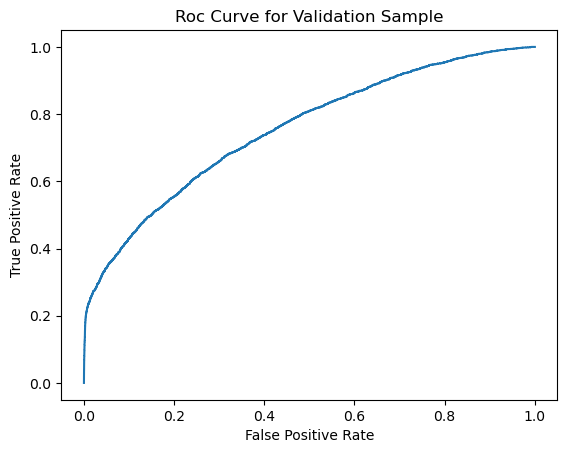
\includegraphics{plots/RF_base_roc.png}
\caption{roc curve}
\end{figure}

Wartość gini dla tego modelu wynosiła około \texttt{0.5}

\hypertarget{strojenie-hiperparametruxf3w}{%
\subsubsection{Strojenie
hiperparametrów}\label{strojenie-hiperparametruxf3w}}

Przy użyciu podstawowych metod wyszukiwania najlepszych hiperparametrów,
takich jak grid oraz random search wytrenowaliśmy model sprawujący się
lepiej na danych treningowych. Korzystając z własności lasów losowych
wiedzieliśmy, że w tym przypadku nie musimy się znacząco przejmować
przetrenowaniem tego modelu, ze względu na odporność lasów losowych na
tak zwany \emph{overfitting}.

W trakcie poszukiwania najlepszego modelu za pomocą zestawów
hiperparametrów stosowaliśmy różne miary jakości modelów, ale
ostatecznie stwierdziliśmy, że modele będą porównywane za pomocą
\emph{balanced accuracy}, aby niezbalansowanie klas nie stanowiło aż tak
dużego problemu.

Jako jedną z miar jakości otrzymanego w ten sposób modelu zastosowaliśmy
ponownie krzywą ROC, pokazującą stosunek czułości (ang. sensitivity) do
specyficzności (ang. specificity).

\begin{figure}
\centering
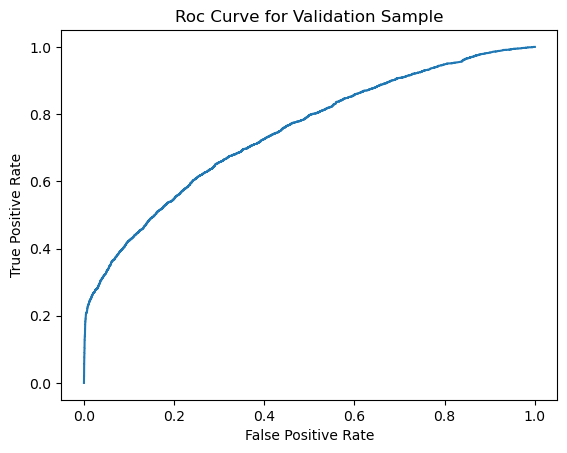
\includegraphics{plots/RF_random_roc.png}
\caption{roc curve}
\end{figure}

Wartość gini dla tego modelu wynosiła również około 0.5, ale mniej niż w
poprzednim przypadku.

Ostatecznie model lasu losowego, który wybraliśmy, miał wartość
wskaźnika \texttt{accuracy} rzędu ponad 90\%. Jednak z uwagi na to, że
klasa pozytywna była niezbyt liczna - w naszym zbiorze danych stosunek
samochodów, które były złym zakupem do tych, które były dobrym był
naprawdę mały. W związku z tym nie był to główny wskaźnik, który
braliśmy pod uwagę.

\hypertarget{rozwiux105zanie-niedoreprezentowania-klasy-samochoduxf3w-uszkodzonych}{%
\subsubsection{Rozwiązanie niedoreprezentowania klasy samochodów
uszkodzonych}\label{rozwiux105zanie-niedoreprezentowania-klasy-samochoduxf3w-uszkodzonych}}

Ponieważ jedynie 12\% samochodów w całym zbiorze danych stanowiło te
będące złym zakupem, próbowaliśmy znaleźć rozwiązanie tego problemu na
różne sposoby.

Zastosowaliśmy różne metody samplowania danych oraz strojenie
hiperparametrów. Rezultaty poprawiły jakość modelu, ale tylko
nieznacznie.

\hypertarget{ocena-predykcyjnoux15bci-cech}{%
\subsubsection{Ocena predykcyjności
cech}\label{ocena-predykcyjnoux15bci-cech}}

W ramach tego modelu sprawdziliśmy również feature importance na dwa
sposoby - za pomocą wbudowanej funkcji lasu losowego
\texttt{feature\_importance\_}, a także za pomocą pakietu
\texttt{shapely}.

Jak się okazało najbardziej istotną kolumną predykcyjną była kolumna
oznaczająca powiązana z WheelTypeID - zmienną określającą rodzaj
kołpaków zamontowanych w samochodzie. Co istotniejsze, nie istnieje
żaden konkretny typ kołpaków, który zwiększałby prawdopodobieństwo
przynależności samochodu do klasy zakupu narażonego na straty. Jak się
okazuje, najwięcej informacji na temat tego czy samochód jest
przysłowiową \emph{cytryną} można było wywnioskować z faktu, czy typ
kołpaka danego samochodu zawierał brak danych. W zależności od
parametrów, predykcyjność takiej kolumny wynosiła nawet do 60\%.

Obserwacja ta nie była przez nas początkowo zauważona. Istotne
wgłębienie się w problem i dokładne przeanalizowanie danych pozwoliło
nam zauważyć przeoczoną, ale bardzo ważną informację dla sprawowania się
modelu, co automatycznie zwiększyło predykcyjność wszystkich naszych
modelów.

\begin{figure}
\centering
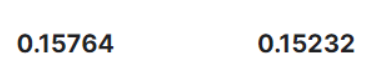
\includegraphics{raport_files/image.png}
\caption{image.png}
\end{figure}

Pozostałymi cechami samochodów, które dawały dużo informacji o tym, czy
zakup był dobry lub nie, były między innymi wiek samochodu, jego cena, a
także wartość ubezpieczenia auta.

\hypertarget{ostateczny-wynik-na-danych-z-kaggle}{%
\subsubsection{Ostateczny wynik na danych z
kaggle}\label{ostateczny-wynik-na-danych-z-kaggle}}

\begin{figure}
\centering
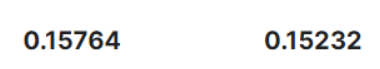
\includegraphics{raport_files/image-2.png}
\caption{image-2.png}
\end{figure}

    \hypertarget{xgboost}{%
\section{XGBoost}\label{xgboost}}

\hypertarget{opis-dziaux142ania}{%
\subsubsection{Opis działania}\label{opis-dziaux142ania}}

XGBoost (eXtreme Gradient Boosting) to potężny algorytm uczenia
maszynowego używany do klasyfikacji i regresji. Opiera się na technice
gradient boosting, łączącej wiele słabych modeli w celu stworzenia
silnego modelu. Działanie XGBoost obejmuje inicjalizację modelu,
obliczanie predykcji początkowych, obliczanie reszt, budowę drzewa,
aktualizację wag, aktualizację predykcji i kontynuację uczenia.
Ostatecznie, model XGBoost generuje predykcje dla nowych danych na
podstawie cech tych danych.

\hypertarget{opis-modelu}{%
\subsubsection{Opis modelu}\label{opis-modelu}}

Zdecydowaliśmy się ponownie użyć grid-search'a, aby znaleźć najlepsze
hiperparametry modelu XGboost.\\
Jak się okazało najlepszy model przy cross-validation=3 sprawdził się
XGBoost z następującymi parametrami:

\{`subsample': 1.0, `n\_estimators': 150, `max\_depth': 5,
`learning\_rate': 0.1, `gamma': 5, `colsample\_bytree': 1.0\}

Dla modelu z powyższymi parametrami obliczyliśmy różne metryki na
zbiorze testowym, które przedstawiają się następująco.\\
Dla klasy 0: precision: 0.88, recall: 0.99\\
Dla klasy 1: precision: 0.39, recall: 0.02\\
Accuracy: 0.88\\

\hypertarget{wizualizacje}{%
\subsubsection{Wizualizacje}\label{wizualizacje}}

A jeżeli chodzi o macierz pomyłek to wygląda ona następująco:

\begin{figure}
\centering
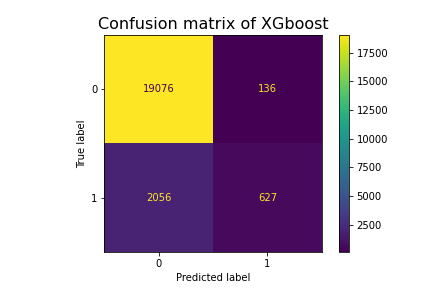
\includegraphics{plots/conf-mat-xgboost.png}
\caption{Confusion Matrix}
\end{figure}

A krzywe roc tak:

Dla danych treningowych:

\begin{figure}
\centering
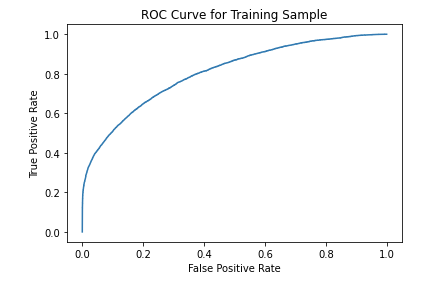
\includegraphics{plots/roc_train_xgboost.png}
\caption{Roc xgb}
\end{figure}

Gini wynosi tutaj 0.61

Dla danych testowych:

\begin{figure}
\centering
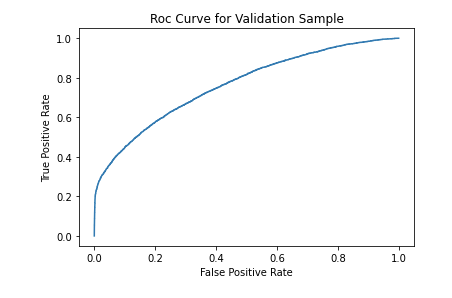
\includegraphics{plots/roc_test_xgboost.png}
\caption{Roc xgb test}
\end{figure}

A tutaj wartość gini 0.52

    \hypertarget{voting-classifier}{%
\section{Voting classifier}\label{voting-classifier}}

\hypertarget{opis-dziaux142ania}{%
\subsubsection{Opis działania}\label{opis-dziaux142ania}}

Klasyfikator głosujący to jedna z technik uczenia zespołowego, która
polega na łączeniu predykcji kilku różnych modeli w celu podjęcia
końcowej decyzji. Działa na zasadzie głosowania, gdzie każdy model
oddaje swój głos na przewidywaną klasę. Istnieją trzy główne typy
głosowania: hard voting, soft voting i weighted voting. W hard voting,
klasa otrzymująca największą liczbę głosów jest wybierana jako końcowa
decyzja. W soft voting, modele przewidują prawdopodobieństwa
przynależności do poszczególnych klas, a ostateczna decyzja jest oparta
na agregacji tych prawdopodobieństw. W weighted voting, nadawane są wagi
poszczególnym modelom, które wpływają na ostateczne głosowanie.

\hypertarget{opis-modelu}{%
\subsubsection{Opis modelu}\label{opis-modelu}}

Do głosowania użyliśmy modeli regresji logistycznej, drzewa decyzyjnego,
lasu losowego oraz xgboost z wybranymi wcześniej najlepszymi
hiperparametrami. W naszym modelu użyliśmy metody soft voting. Za pomocą
losowego przeszukiwania siatki wybraliśmy również najbardziej korzystny
pod względem dokładności zestaw wag charakteryzujący stosunek istotności
głosu każdego modelu w głosowaniu. Nalepsze rezultaty otrzymaliśmy
uwzględniając jedynie las losowy oraz xgboost. Wyniki są bardzo
zadowalające - 90.09\% dokładności oraz 84.08\% precyzji dla zbioru
walidacyjnego, przy jednoczesnym braku oznak przetrenowania modelu.

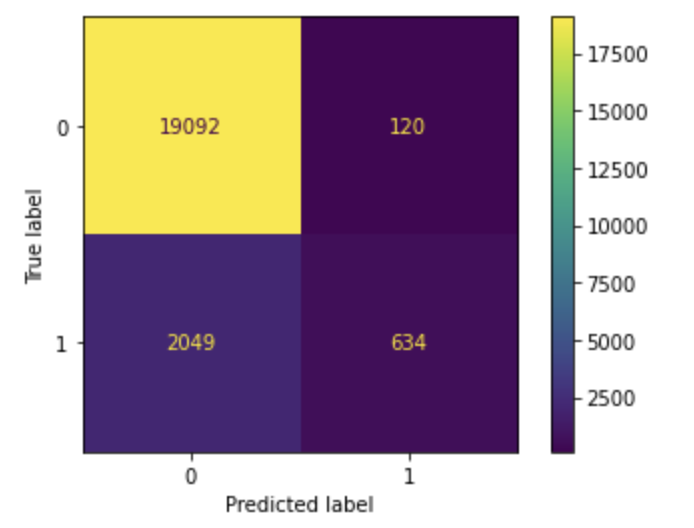
\includegraphics{plots/voting_confusion.png}

\hypertarget{wizualizacje}{%
\subsubsection{Wizualizacje}\label{wizualizacje}}

Krzywa roc oraz rezultat gini dla zbioru walidacyjnego kształtują się na
poziomie modeli lasu losowego i xgboost:

Dla danych treningowych: gini = 0.8682

\begin{figure}
\centering
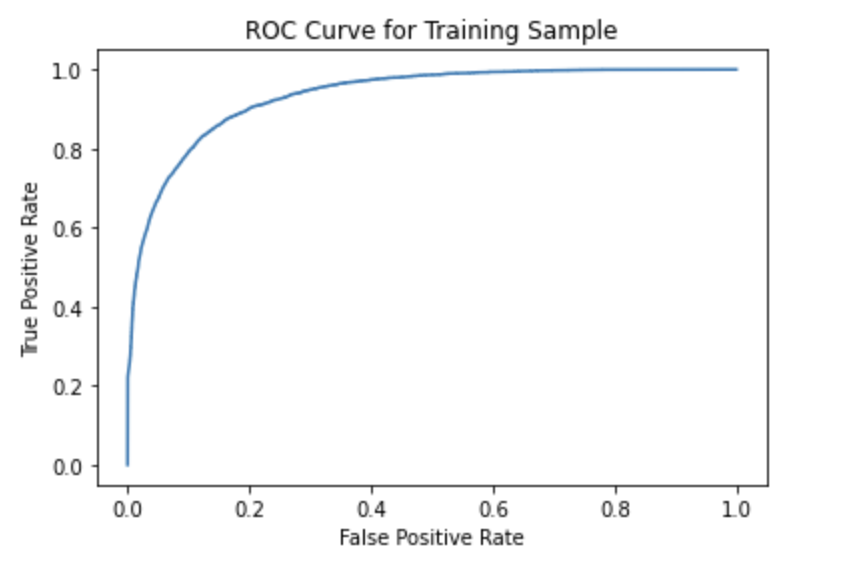
\includegraphics{plots/voting_roc_train.png}
\caption{reg\_coef}
\end{figure}

Dla danych walidacyjnych: gini = 0.5256

\begin{figure}
\centering
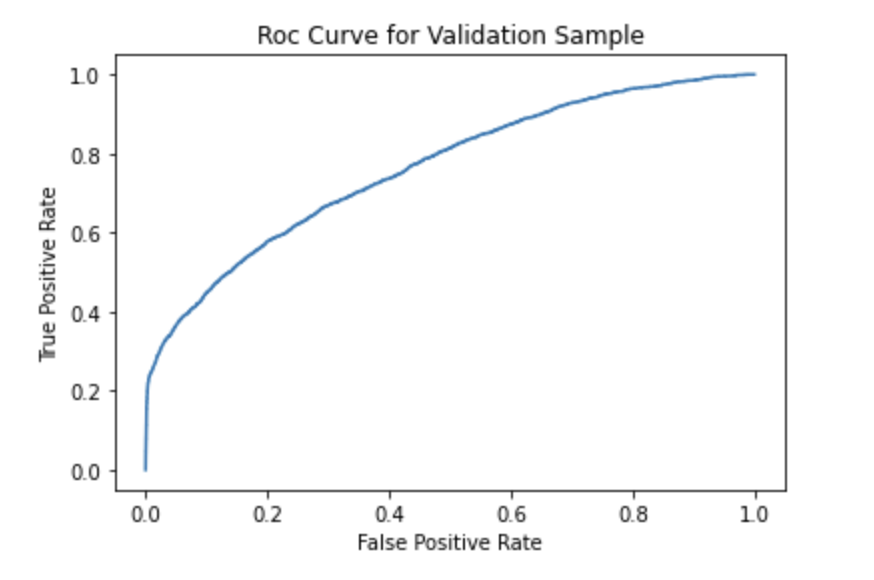
\includegraphics{plots/voting_roc_val.png}
\caption{reg\_coef}
\end{figure}

    \hypertarget{svm}{%
\subsection{SVM}\label{svm}}

\hypertarget{opis-dziaux142ania}{%
\subsubsection{Opis działania}\label{opis-dziaux142ania}}

SVM (Support Vector Machines) to algorytm uczenia maszynowego, który
znajduje optymalną hiperpłaszczyznę separującą dane różnych klas. Działa
poprzez wybór hiperpłaszczyzny, wyszukiwanie optymalnej z maksymalnym
marginesem, wykorzystanie kernel tricku do przekształcenia danych do
przestrzeni separowalnej liniowo lub nieliniowo, optymalizację modelu i
klasyfikację nowych danych na podstawie ich położenia względem
hiperpłaszczyzny. SVM jest skuteczny dla danych z wieloma cechami i
potrafi radzić sobie z danymi nieliniowo separowalnymi.

\hypertarget{opis-modelu}{%
\subsubsection{Opis modelu}\label{opis-modelu}}

Niestety okazało się, że model ten nie dość, że bardzo długo się
trenował, to także słabo się sprawdził. Był to model, którego accuracy
można by było porównać do DummyClassifier, ponieważ prawie wszystkie
wiersze przydzielał do klasy 1. Z tego też powodu nie załączam tu
żadnych więcej metryk, gdyź byłoby to po prostu zbędne. Warto też
wspomnieć, że może to mieć coś wspólnego ze skalą cech (mimo że
normalizowaliśmy większość kolumn).

    \hypertarget{rozwiux105zanie-niedoreprezentowania-klasy-samochoduxf3w-uszkodzonych}{%
\subsection{Rozwiązanie niedoreprezentowania klasy samochodów
uszkodzonych}\label{rozwiux105zanie-niedoreprezentowania-klasy-samochoduxf3w-uszkodzonych}}

Ponieważ jedynie 12\% samochodów w całym zbiorze danych stanowiło te
będące złym zakupem, próbowaliśmy znaleźć rozwiązanie tego problemu na
różne sposoby.

Przetestowaliśmy różne sposoby radzenia sobie z tym problemem pochodzące
z książki autorstwa Max Kuhna oraz Kjell Johnson \emph{Applied
Predictive Modeling}.

Wśród rozwiązań, które zastosowaliśmy były między innymi odpowiednie
strojenie hiperparametrów (za pomocą metod przeszukiwania siatki
hiperparametrów i innych), próbowaliśmy w ten sposób zmaksymalizować
różne wskaźniki jakości modelów - nie tylko najczęściej stosowane
\emph{accuracy}. Ta metoda okazała się jednak nieskuteczna w naszym
przypadku.

Innym podejściem, które staraliśmy się zastosować były metody
\emph{samplowania} danych. Staraliśmy się modyfikować sztucznie zbiór
danych testowych, tak aby proporcje pomiędzy klasami były zrównoważone.
Stosując tę technikę dla modelu \texttt{XGBoost} modele trenowane na
upsamplowanych danych okazały się znacznie gorsze niż te trenowane na
orginalnych danych. W przypadku modelów lasów losowych technika SMOTE
okazała się poprawiać w pewnym stopniu wyniki modelów na zbiorze
walidacyjnym, kosztem jednak znacznie dłuższego czasu potrzebnego do
wytrenowania modeli.

Jak się jednak okazało, wytrenowany las losowy z użyciem SMOTE w
konkursie na kagglu osiągnął najlepszy wynik.

W przypadku XGboosta metoda oversamplingu nie spisała się najlepiej,
gdyż wartość test accuracy spadła do 68.35, gdzie w modelu bez
oversamplingu wartość ta wynosiła 87.69.

    \hypertarget{podsumowanie}{%
\section{Podsumowanie}\label{podsumowanie}}

Wykonując testy za pomocą algorytmu \emph{kaggle'a} na zbiorze testowym
uzyskaliśmy przyzwoite rezultaty w porównaniu do pozostałych zawodników
biorących udział w już zakończonych zawodach. Nasz najlepszy wynik
osiągnięty za pomocą modelu lasu losowego dał nam satysfakcjonujący
wynik.

\begin{figure}
\centering
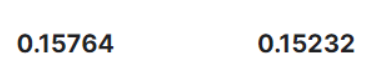
\includegraphics{raport_files/image.png}
\caption{image.png}
\end{figure}

Nie pozwoliłby nam on wygrać zawodów, ale ten uznaliśmy go za bardzo
dobry, biorąc pod uwagę nasze doświadczenie w tego typu projektach .
Zaczynając pracę nad projektem, żaden z nas nie miał doświadczenia w
dziedzinie uczenia maszynowego.

Dzięki temu, w trakcie pracy nad projektem nie tylko udało nam się
zbudować wiele modeli i osiągnąć założone cele biznesowe. Udało nam się
ustalić, które cechy były najbardziej istotne dla naszych modelów, a co
więcej, różne modele zwracały te same wyniki. Co więcej udało się
wytrenować las losowy w ten sposób, aby liczba obserwacji False Negative
była niewielka. Ostatecznie, co najważniejsze, udało sie nam również
sporo się nauczyć.


    % Add a bibliography block to the postdoc
    
    
    
\end{document}
